\documentclass[11pt,letterpaper]{article}

\usepackage[utf8]{inputenc}
\usepackage[T1]{fontenc}
\usepackage[spanish]{babel}
\usepackage{graphicx}
\usepackage{geometry}
\usepackage{amsmath}
\usepackage{listings}
\usepackage{xcolor}
\usepackage{float}
\usepackage[hidelinks]{hyperref}

\geometry{letterpaper, margin=2.1cm}

\lstset{
    language=Python,
    basicstyle=\ttfamily\footnotesize,
    keywordstyle=\color{blue},
    commentstyle=\color{gray},
    stringstyle=\color{red!60!black},
    numbers=left,
    numberstyle=\tiny,
    frame=single,
    breaklines=true,
    showstringspaces=false,
    columns=fullflexible
}

\title{Taller 3: Ecualización y Transformaciones de Intensidad}
\author{
Camilo Eduardo Muñoz Albornoz\\
Procesamiento Digital de Imágenes\\
Universidad Tecnológica de Pereira
}
\date{}

\begin{document}

\maketitle

\begin{center}
\textbf{Código fuente en GitHub}\\[0.2cm]
\textbf{Cuaderno o programa Python: }\href
{https://github.com/CamiloMunozAL/ProcDImagenes/blob/main/taller3/taller3.ipynb}
{\textcolor{blue}{\underline{\texttt{github.com/CamiloMunozAL/ProcDImagenes/blob/main/taller3/taller3.ipynb}}}}\\[0.15cm]
\textbf{Carpeta del Taller 3: }\href
{https://github.com/CamiloMunozAL/ProcDImagenes/tree/main/taller3}
{\textcolor{blue}{\underline{\texttt{github.com/CamiloMunozAL/ProcDImagenes/tree/main/taller3}}}}
\end{center}

\begin{abstract}
En este taller se estudiaron diferentes técnicas para modificar la distribución de intensidades de imágenes digitales mediante ecualización de histograma y transformaciones lineales y no lineales. Se trabajó con imágenes en escala de grises y a color utilizando Python, OpenCV y NumPy. Se analizaron operaciones de ecualización automática, oscurecimiento, aclarado, reducción y aumento de contraste, y una transformación gamma aplicada independientemente a los canales de color. Los histogramas permitieron observar cómo cada operación modifica la distribución de los niveles de intensidad y, por consiguiente, la apariencia de la imagen.
\end{abstract}


% =========================================================
\section{Objetivos y preguntas del taller}

El objetivo general fue comprender cómo las transformaciones de intensidad permiten modificar el brillo y el contraste de una imagen, y analizar dichos cambios mediante sus histogramas.

El taller desarrollado corresponde a los siguientes puntos:

\begin{enumerate}
    \item Ecualizar una imagen en escala de grises utilizando la función proporcionada por OpenCV.
    
    \item Comparar los histogramas de la imagen original y la imagen ecualizada.
    
    \item Oscurecer los píxeles de la imagen original a una tercera parte de su intensidad.
    
    \item Aclarar la imagen original al menos un 30\%.
    
    \item Aplicar una transformación para producir una imagen de bajo contraste.
    
    \item Aplicar una transformación para producir una imagen de alto contraste.
    
    \item Aplicar una transformación lineal o no lineal sobre cada canal de una imagen a color.
\end{enumerate}


% =========================================================
\section{Fundamento teórico}

\subsection{Transformaciones de intensidad}

En una imagen digital en escala de grises de 8 bits, cada píxel posee una intensidad entre 0 y 255:

\begin{equation}
0 \leq x \leq 255
\end{equation}

donde 0 representa negro, 255 representa blanco y los valores intermedios corresponden a diferentes niveles de gris.

Una transformación de intensidad toma el valor original de un píxel $x$ y calcula un nuevo valor $y$:

\begin{equation}
y=T(x)
\end{equation}

Por ejemplo, si se utiliza:

\begin{equation}
y=\frac{x}{3}
\end{equation}

un píxel con intensidad 180 pasa a tener intensidad 60, por lo que se vuelve más oscuro.

En general:

\begin{itemize}
    \item Si $y<x$, el píxel se oscurece.
    \item Si $y>x$, el píxel se aclara.
    \item Si $y=x$, el píxel no cambia.
\end{itemize}

Cuando una operación genera valores por fuera del intervalo $[0,255]$, estos deben limitarse. Este procedimiento se conoce como \textit{clipping} o saturación:

\begin{equation}
y=
\begin{cases}
0, & y<0\\
y, & 0\leq y\leq255\\
255, & y>255
\end{cases}
\end{equation}


\subsection{Histograma y contraste}

El histograma representa la cantidad de píxeles existentes en cada nivel de intensidad.

Una imagen de bajo contraste suele utilizar solamente una región reducida del intervalo $0$--$255$. Por el contrario, una imagen con mayor contraste presenta una separación mayor entre las intensidades oscuras y claras.

Por esta razón:

\begin{itemize}
    \item Comprimir el rango de intensidades disminuye el contraste.
    \item Expandir el rango de intensidades aumenta el contraste.
\end{itemize}


\subsection{Ecualización de histograma}

La ecualización de histograma es una técnica que redistribuye los niveles de intensidad buscando aprovechar mejor el rango disponible y mejorar el contraste global.

Para realizar esta transformación se utiliza la distribución acumulada del histograma o CDF (\textit{Cumulative Distribution Function}). De forma simplificada:

\begin{equation}
s_k=(L-1)\,CDF(k)
\end{equation}

donde:

\begin{itemize}
    \item $k$ representa una intensidad original,
    \item $L$ es el número de niveles posibles,
    \item para una imagen de 8 bits, $L=256$.
\end{itemize}

Por tanto:

\begin{equation}
s_k=255\,CDF(k)
\end{equation}

La ecualización no necesariamente produce un histograma perfectamente uniforme. Debido a la naturaleza discreta de una imagen digital, algunos niveles pueden quedar vacíos y otros pueden acumular varios valores originales.


\subsection{Transformación gamma}

La corrección gamma es una transformación no lineal cuya forma general es:

\begin{equation}
y=cx^\gamma
\end{equation}

donde:

\begin{itemize}
    \item $x$ es la intensidad original,
    \item $y$ es la intensidad transformada,
    \item $\gamma$ controla la forma de la transformación,
    \item $c$ es una constante de escala.
\end{itemize}

Para trabajar de forma conveniente con imágenes de 8 bits se normalizan primero las intensidades al intervalo $[0,1]$:

\begin{equation}
x_n=\frac{x}{255}
\end{equation}

Luego:

\begin{equation}
y_n=x_n^\gamma
\end{equation}

y finalmente se regresa al intervalo $[0,255]$:

\begin{equation}
y=255\left(\frac{x}{255}\right)^\gamma
\end{equation}

Cuando:

\begin{itemize}
    \item $\gamma<1$, las intensidades bajas y medias aumentan y la imagen se aclara.
    \item $\gamma=1$, la imagen permanece sin cambios.
    \item $\gamma>1$, las intensidades disminuyen y la imagen se oscurece.
\end{itemize}


% =========================================================
\section{Desarrollo del taller}


% =========================================================
\subsection{Punto 1: Ecualización de una imagen en escala de grises}

\textbf{Procedimiento.}

La imagen \texttt{paisaje.png} fue cargada en escala de grises y posteriormente se aplicó la función \texttt{cv2.equalizeHist()} de OpenCV:

\begin{lstlisting}
imagen_gris = cv2.imread(
    "images/paisaje.png",
    cv2.IMREAD_GRAYSCALE
)

imagen_ecualizada = cv2.equalizeHist(
    imagen_gris
)
\end{lstlisting}

Esta operación no modifica las dimensiones de la imagen, sino los valores de intensidad de sus píxeles.

\begin{figure}[H]
    \centering
    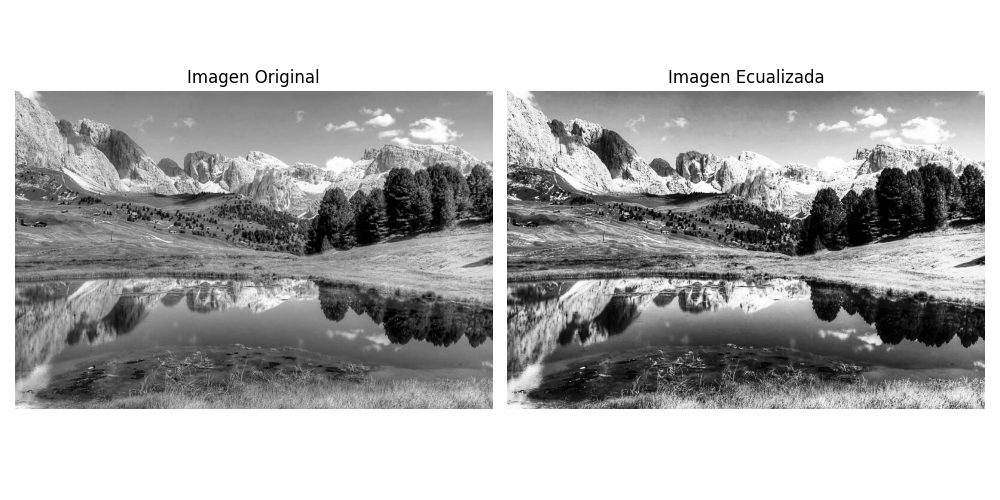
\includegraphics[width=\textwidth]
    {../resultados/imagen_ecualizada.png}
    \caption{Comparación entre la imagen original y la imagen ecualizada.}
    \label{fig:imagen-ecualizada}
\end{figure}

\textbf{Resultado.}

Como se observa en la
\hyperref[fig:imagen-ecualizada]{Figura~\ref*{fig:imagen-ecualizada}},
la imagen ecualizada presenta una mayor separación entre regiones oscuras y claras. Se hacen más evidentes detalles de las montañas, árboles, terreno y reflejos.

Los valores obtenidos fueron:

\begin{itemize}
    \item Intensidad mínima original: 0.
    \item Intensidad máxima original: 255.
    \item Promedio original: 126.18.
    \item Intensidad mínima ecualizada: 0.
    \item Intensidad máxima ecualizada: 255.
    \item Promedio ecualizado: 127.33.
\end{itemize}

Es importante observar que el rango ya era $0$--$255$ antes de la operación. Por tanto, el aumento de contraste no se produjo simplemente por ampliar el mínimo y máximo, sino por redistribuir los píxeles dentro de ese intervalo.


% =========================================================
\subsection{Punto 2: Comparación de histogramas}

Para analizar la modificación producida por la ecualización se calcularon los histogramas de ambas imágenes:

\begin{lstlisting}
histograma_original = cv2.calcHist(
    [imagen_gris], [0], None,
    [256], [0, 256]
)

histograma_ecualizado = cv2.calcHist(
    [imagen_ecualizada], [0], None,
    [256], [0, 256]
)
\end{lstlisting}

\begin{figure}[H]
    \centering
    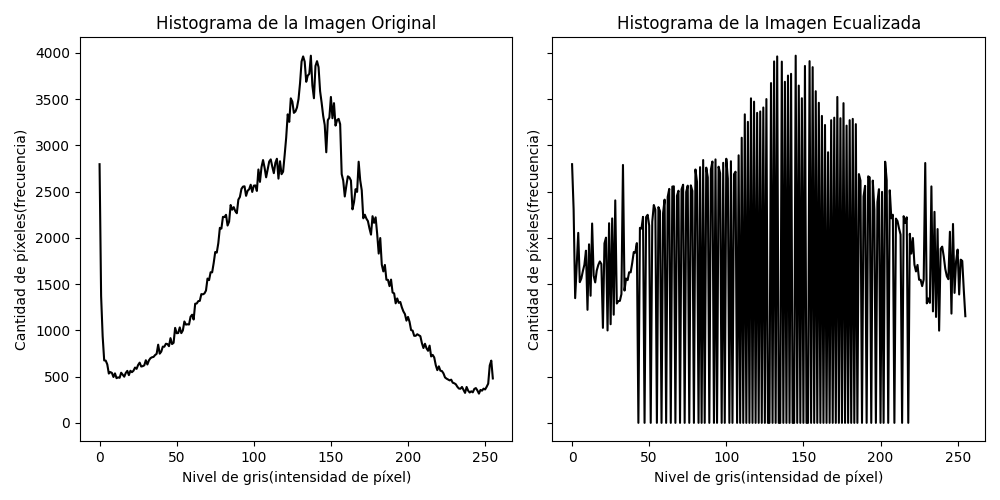
\includegraphics[width=\textwidth]
    {../resultados/histogramas_ecualizados.png}
    \caption{Comparación de los histogramas antes y después de la ecualización.}
    \label{fig:histogramas-ecualizados}
\end{figure}

En el histograma original de la
\hyperref[fig:histogramas-ecualizados]{Figura~\ref*{fig:histogramas-ecualizados}}
se observa una concentración importante de píxeles en niveles medios, principalmente alrededor de las intensidades 100--180.

Después de la ecualización los valores se distribuyen a lo largo de una parte mayor del rango disponible. También aparecen niveles con frecuencia cero, visibles como separaciones entre los picos.

Estos espacios no representan un error. La transformación asigna los niveles originales a nuevos valores enteros y algunos niveles de salida pueden quedar sin utilizar.


% =========================================================
\subsection{Punto 3: Oscurecimiento a una tercera parte}

Para disminuir el brillo se aplicó a cada píxel la transformación:

\begin{equation}
y=\frac{x}{3}
\end{equation}

El procedimiento fue implementado recorriendo la imagen:

\begin{lstlisting}
filas, columnas = imagen_gris.shape
imagen_oscura = imagen_gris.copy()

for fila in range(filas):
    for columna in range(columnas):
        pixel_original = int(
            imagen_gris[fila, columna]
        )

        pixel_ecualizado = (
            pixel_original // 3
        )

        imagen_oscura[fila, columna] = (
            pixel_ecualizado
        )
\end{lstlisting}

Luego se calculó el histograma:

\begin{lstlisting}
histograma_oscuro = cv2.calcHist(
    [imagen_oscura], [0], None,
    [256], [0, 256]
)
\end{lstlisting}

\begin{figure}[H]
    \centering
    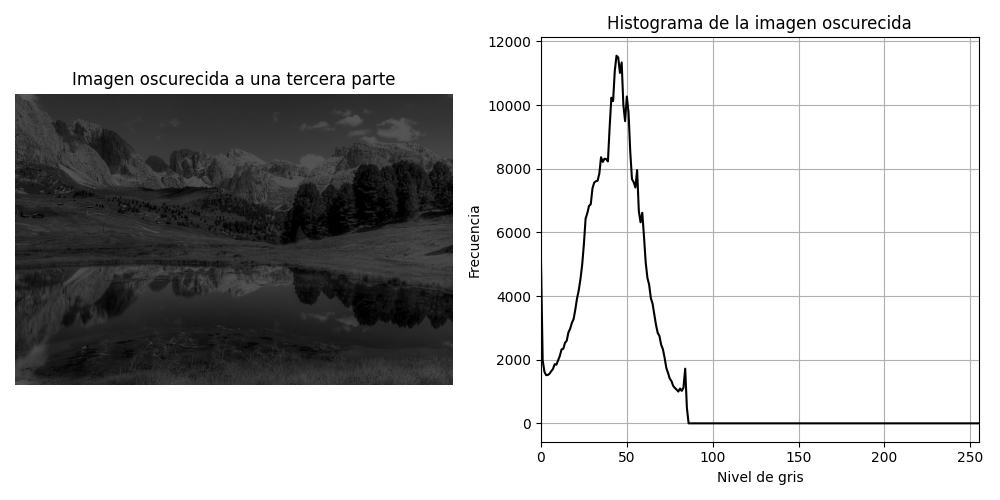
\includegraphics[width=\textwidth]
    {../resultados/imagen_oscurecida_pt3.png}
    \caption{Imagen oscurecida a una tercera parte y su histograma.}
    \label{fig:imagen-oscura}
\end{figure}

Como se observa en la
\hyperref[fig:imagen-oscura]{Figura~\ref*{fig:imagen-oscura}},
el histograma queda concentrado entre 0 y 85.

Esto ocurre porque:

\begin{equation}
\frac{255}{3}=85
\end{equation}

Los resultados obtenidos fueron:

\begin{itemize}
    \item Mínimo original: 0.
    \item Máximo original: 255.
    \item Promedio original: 126.18.
    \item Mínimo oscurecido: 0.
    \item Máximo oscurecido: 85.
    \item Promedio oscurecido: 41.73.
\end{itemize}

La reducción del promedio y la concentración del histograma hacia la izquierda confirman la disminución general del brillo.


% =========================================================
\subsection{Punto 4: Aumento de brillo en un 30\%}

Para aclarar la imagen se aumentó cada intensidad en un 30\%:

\begin{equation}
y=1.3x
\end{equation}

Como esta operación puede generar valores superiores a 255, se utilizó \texttt{np.clip()}:

\begin{lstlisting}
imagen_clara = np.clip(
    imagen_gris * 1.3,
    0,
    255
).astype(np.uint8)
\end{lstlisting}

\begin{figure}[H]
    \centering
    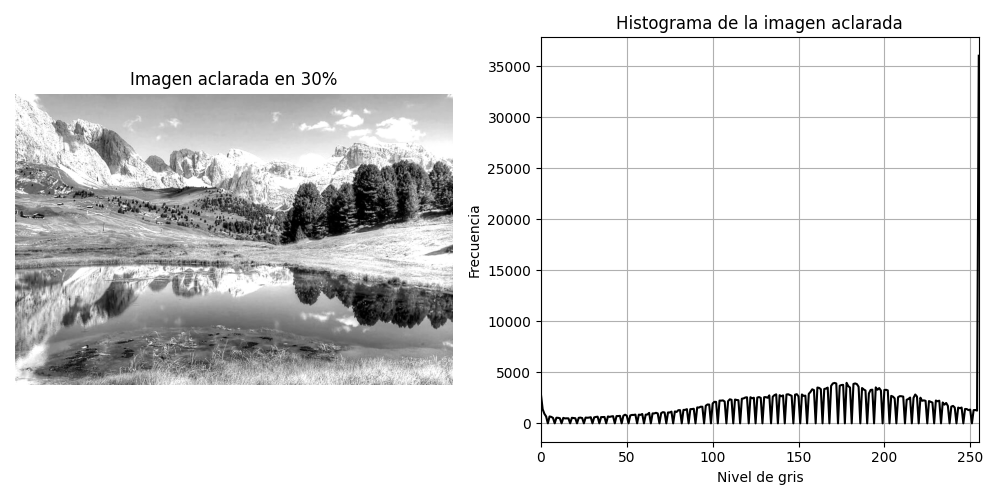
\includegraphics[width=\textwidth]
    {../resultados/imagen_aclarada_pt4.png}
    \caption{Imagen aclarada en un 30\% y su histograma.}
    \label{fig:imagen-clara}
\end{figure}

En la
\hyperref[fig:imagen-clara]{Figura~\ref*{fig:imagen-clara}}
puede observarse el desplazamiento del histograma hacia intensidades mayores.

Los valores obtenidos fueron:

\begin{itemize}
    \item Promedio original: 126.18.
    \item Promedio después del aclarado: 161.06.
    \item Intensidad mínima: 0.
    \item Intensidad máxima: 255.
\end{itemize}

El gran pico ubicado en la intensidad 255 corresponde a los píxeles que, al multiplicarse por 1.3, superaron el máximo permitido y fueron limitados a 255 mediante saturación.


% =========================================================
\subsection{Punto 5: Reducción del contraste}

Para disminuir el contraste se utilizó la transformación:

\begin{equation}
y=0.5x+64
\end{equation}

La implementación fue:

\begin{lstlisting}
imagen_bajo_contraste = np.clip(
    imagen_gris * 0.5 + 64,
    0,
    255
).astype(np.uint8)
\end{lstlisting}

Para $x=0$:

\begin{equation}
y=64
\end{equation}

y para $x=255$:

\begin{equation}
y\approx191
\end{equation}

Por tanto, el rango completo $0$--$255$ queda comprimido aproximadamente al intervalo $64$--$191$.

\begin{figure}[H]
    \centering
    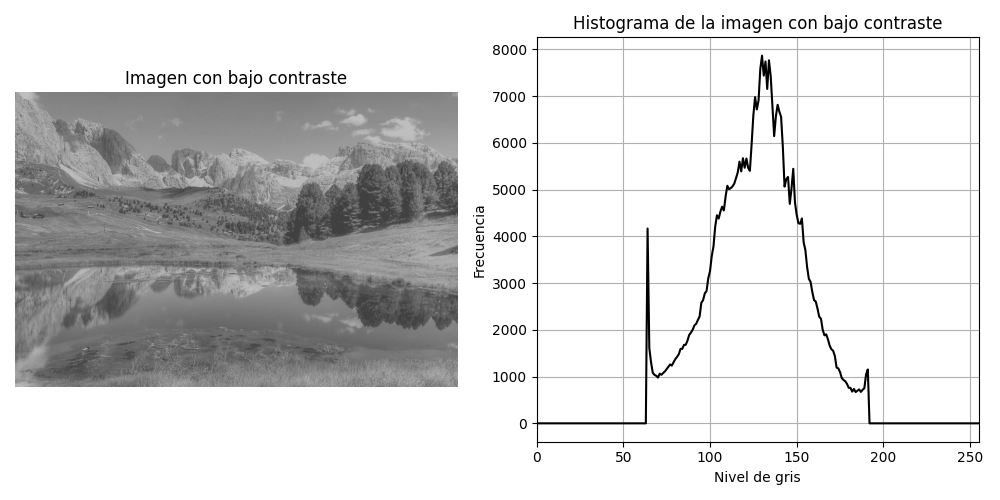
\includegraphics[width=\textwidth]
    {../resultados/imagen_bajo_contraste_pt5.png}
    \caption{Imagen con bajo contraste y distribución de intensidades resultante.}
    \label{fig:bajo-contraste}
\end{figure}

La
\hyperref[fig:bajo-contraste]{Figura~\ref*{fig:bajo-contraste}}
muestra que el histograma queda concentrado en una zona más estrecha y central.

Los resultados fueron:

\begin{itemize}
    \item Mínimo: 64.
    \item Máximo: 191.
    \item Promedio: 126.84.
\end{itemize}

El promedio permanece próximo al original, pero desaparecen los negros y blancos extremos. Visualmente, la imagen adquiere una apariencia más gris o ``lavada'', característica de un contraste reducido.


% =========================================================
\subsection{Punto 6: Aumento del contraste}

Para incrementar el contraste se utilizó:

\begin{equation}
y=2x-128
\end{equation}

La transformación amplía la diferencia de los valores alrededor de las intensidades medias.

Debido a que pueden producirse valores negativos, inicialmente se convirtió la matriz a \texttt{int16}:

\begin{lstlisting}
imagen_alto_contraste = np.clip(
    imagen_gris.astype(np.int16) * 2 - 128,
    0,
    255
).astype(np.uint8)
\end{lstlisting}

La conversión a \texttt{int16} evita problemas de desbordamiento al realizar operaciones negativas sobre datos originalmente almacenados como enteros sin signo de 8 bits.

\begin{figure}[H]
    \centering
    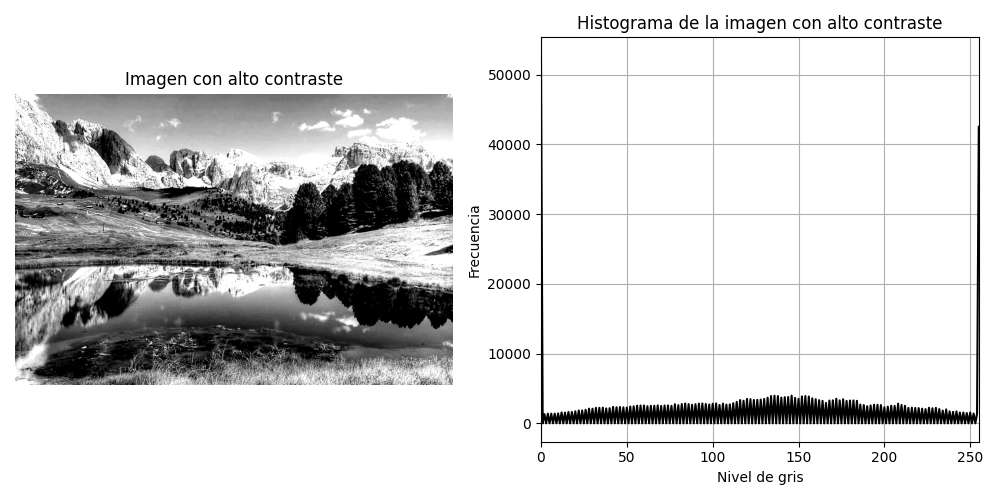
\includegraphics[width=\textwidth]
    {../resultados/imagen_alto_contraste_pt6.png}
    \caption{Imagen con alto contraste y su histograma.}
    \label{fig:alto-contraste}
\end{figure}

Como se aprecia en la
\hyperref[fig:alto-contraste]{Figura~\ref*{fig:alto-contraste}},
las zonas oscuras se vuelven más oscuras y las claras más claras.

Los resultados fueron:

\begin{itemize}
    \item Mínimo: 0.
    \item Máximo: 255.
    \item Promedio: 126.77.
\end{itemize}

Los picos observados en 0 y 255 se producen porque los valores que quedan por debajo de 0 o por encima de 255 son saturados en estos extremos. Esto aumenta visualmente la separación entre regiones claras y oscuras.


% =========================================================
\subsection{Punto 7: Transformación gamma sobre una imagen a color}

Para este punto se seleccionó una transformación no lineal mediante corrección gamma, utilizando:

\begin{equation}
\gamma=0.5
\end{equation}

La imagen fue normalizada al intervalo $[0,1]$, se aplicó la potencia y posteriormente se regresó al intervalo $[0,255]$:

\begin{lstlisting}
gamma = 0.5

imagen_color = cv2.imread(
    "images/paisaje.png",
    cv2.IMREAD_COLOR
)

imagen_normalizada = (
    imagen_color / 255.0
)

imagen_gamma = 255 * (
    imagen_normalizada ** gamma
)

imagen_gamma = np.clip(
    imagen_gamma,
    0,
    255
).astype(np.uint8)
\end{lstlisting}

Matemáticamente:

\begin{equation}
y=
255
\left(
\frac{x}{255}
\right)^{0.5}
\end{equation}

Al utilizar $\gamma<1$, los valores bajos y medios aumentan más que los valores que ya se encontraban cerca de 255.

Por ejemplo:

\begin{equation}
64
\rightarrow
255
\left(
\frac{64}{255}
\right)^{0.5}
\approx128
\end{equation}

Por tanto, una intensidad inicialmente baja puede aumentar considerablemente.

\begin{figure}[H]
    \centering
    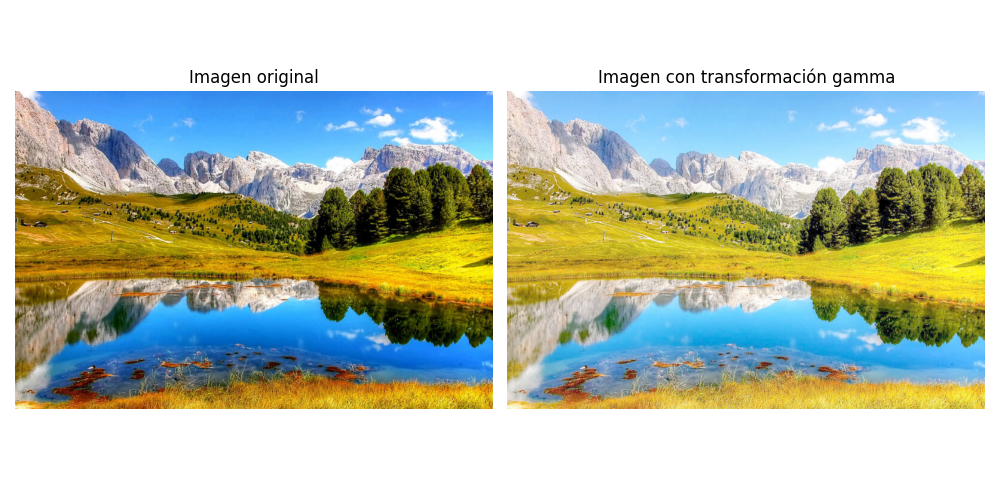
\includegraphics[width=\textwidth]
    {../resultados/gamma_color_pt7.png}
    \caption{Comparación entre la imagen original y la imagen con transformación gamma $\gamma=0.5$.}
    \label{fig:gamma-color}
\end{figure}

Como se observa en la
\hyperref[fig:gamma-color]{Figura~\ref*{fig:gamma-color}},
la imagen resultante es más clara, principalmente en regiones que originalmente presentaban intensidades bajas y medias.


\subsubsection{Análisis por canales}

OpenCV almacena las imágenes a color en orden BGR:

\begin{equation}
P(i,j)=[B,G,R]
\end{equation}

Por esta razón se separaron los tres canales de la imagen original y transformada:

\begin{lstlisting}
blue_original = imagen_color[:, :, 0]
green_original = imagen_color[:, :, 1]
red_original = imagen_color[:, :, 2]

blue_transformado = imagen_gamma[:, :, 0]
green_transformado = imagen_gamma[:, :, 1]
red_transformado = imagen_gamma[:, :, 2]
\end{lstlisting}

Posteriormente se calculó el histograma de cada canal. Por ejemplo:

\begin{lstlisting}
hist_blue_original = cv2.calcHist(
    [blue_original], [0], None,
    [256], [0, 256]
)

hist_blue_transformado = cv2.calcHist(
    [blue_transformado], [0], None,
    [256], [0, 256]
)
\end{lstlisting}

El mismo procedimiento se aplicó a los canales verde y rojo.

\begin{figure}[H]
    \centering
    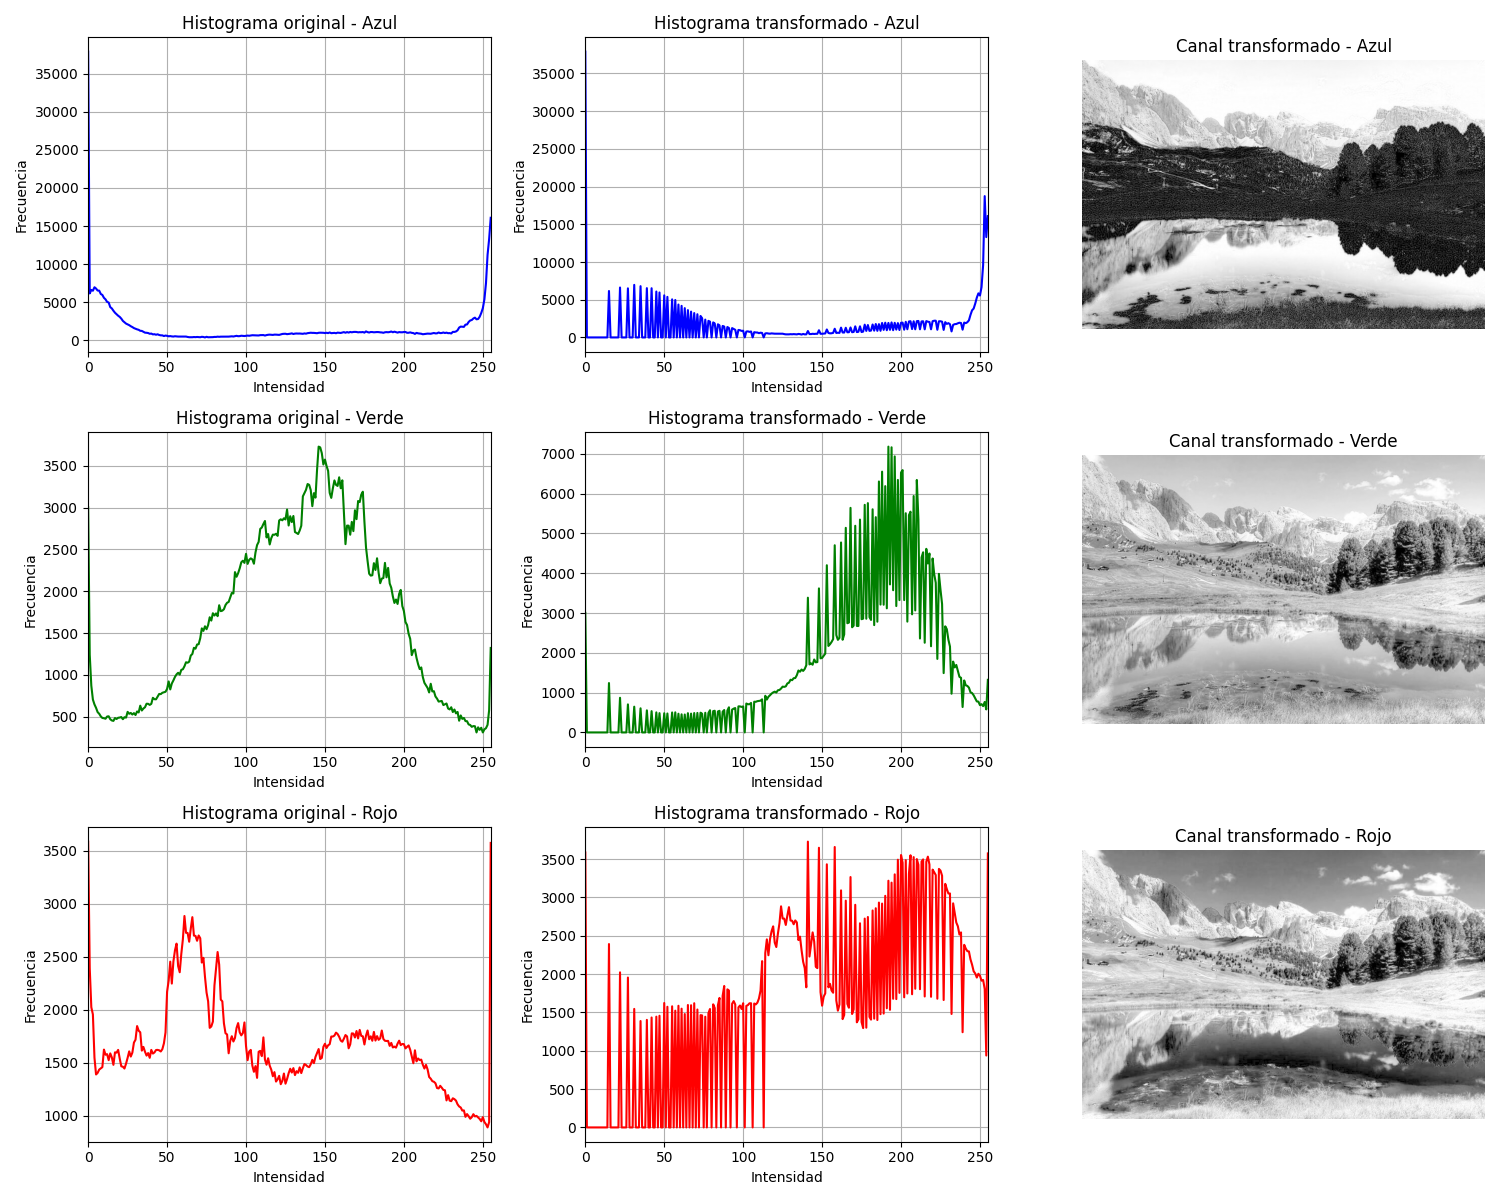
\includegraphics[width=\textwidth]
    {../resultados/canales_gamma_pt7.png}
    \caption{Comparación de histogramas originales y transformados y representación de cada canal después de aplicar gamma.}
    \label{fig:gamma-canales}
\end{figure}

En la
\hyperref[fig:gamma-canales]{Figura~\ref*{fig:gamma-canales}}
se observa que los histogramas de los tres canales se desplazan hacia intensidades mayores.

El efecto es especialmente visible en intensidades bajas y medias, mientras que los valores cercanos a 255 presentan una modificación menor. Este comportamiento es propio de una transformación con $\gamma<1$.

Los histogramas transformados también presentan diversos picos y niveles de intensidad sin frecuencia. Esto se debe a que la transformación no lineal produce inicialmente valores decimales que posteriormente deben cuantizarse nuevamente a valores enteros de 8 bits. Como resultado, varios niveles originales pueden terminar en una misma intensidad y algunos valores de salida pueden quedar sin utilizar.


% =========================================================
\section{Análisis general de resultados}

Los diferentes experimentos permiten observar directamente la relación entre una transformación matemática y el comportamiento del histograma.

En la ecualización mediante \texttt{cv2.equalizeHist}, el rango mínimo y máximo se mantuvo en $0$ y $255$, pero la distribución interna de las intensidades cambió. Esto demuestra que el contraste no depende solamente de los valores extremos, sino de cómo se distribuyen los píxeles entre ellos.

El oscurecimiento a una tercera parte comprimió el rango hasta $0$--$85$ y redujo el promedio de intensidad de 126.18 a 41.73. En consecuencia, el histograma se desplazó notablemente hacia la izquierda.

En el aclarado del 30\%, el promedio aumentó a 161.06 y el histograma se desplazó hacia la derecha. El pico en 255 permitió identificar directamente el efecto del \textit{clipping}.

La transformación de bajo contraste comprimió el rango al intervalo $64$--$191$, acercando entre sí las intensidades claras y oscuras. La transformación de alto contraste produjo el comportamiento contrario, alejando las intensidades del centro y generando acumulaciones en los extremos.

Finalmente, la corrección gamma permitió comprobar el comportamiento de una transformación no lineal. Con $\gamma=0.5$ los valores oscuros y medios aumentaron de intensidad de forma más pronunciada que los valores altos, generando una imagen más clara sin aplicar un incremento lineal uniforme a todos los píxeles.


% =========================================================
\section{Conclusiones}

Las transformaciones de intensidad permiten modificar de manera controlada el aspecto de una imagen digital mediante operaciones matemáticas aplicadas sobre sus píxeles.

La ecualización de histograma redistribuye las intensidades según su distribución acumulada y puede mejorar el contraste global incluso cuando la imagen original ya utiliza todo el rango $0$--$255$.

Las transformaciones lineales permitieron comprobar que el brillo y el contraste son propiedades diferentes. Multiplicar o dividir las intensidades modifica principalmente el brillo, mientras que comprimir o expandir la separación entre valores modifica el contraste.

Los histogramas resultaron fundamentales para interpretar cada transformación. Un desplazamiento hacia la izquierda estuvo asociado con imágenes más oscuras; un desplazamiento hacia la derecha, con imágenes más claras; una concentración en una región estrecha, con bajo contraste; y una mayor separación de las intensidades, con un contraste más alto.

También se evidenció la importancia de limitar los resultados al intervalo $0$--$255$. El uso de \texttt{np.clip()} evitó valores inválidos y permitió observar el fenómeno de saturación cuando múltiples píxeles alcanzaron los extremos 0 o 255.

Finalmente, la transformación gamma mostró que una operación no lineal puede modificar de manera diferente las intensidades bajas, medias y altas. Con $\gamma=0.5$ se aclararon principalmente las regiones oscuras y medias de los tres canales de color, demostrando que las transformaciones no lineales ofrecen un mayor control sobre la distribución de intensidades que una modificación lineal simple.

\end{document}